%% ****** Start of file apstemplate.tex ****** %
%%
%%
%%   This file is part of the APS files in the REVTeX 4.2 distribution.
%%   Version 4.2a of REVTeX, January, 2015
%%
%%
%%   Copyright (c) 2015 The American Physical Society.
%%
%%   See the REVTeX 4 README file for restrictions and more information.
%%
%
% This is a template for producing manuscripts for use with REVTEX 4.2
% Copy this file to another name and then work on that file.
% That way, you always have this original template file to use.
%
% Group addresses by affiliation; use superscriptaddress for long
% author lists, or if there are many overlapping affiliations.
% For Phys. Rev. appearance, change preprint to twocolumn.
% Choose pra, prb, prc, prd, pre, prl, prstab, prstper, or rmp for journal
%  Add 'draft' option to mark overfull boxes with black boxes
%  Add 'showkeys' option to make keywords appear
%\documentclass[aps,prl,preprint,groupedaddress]{revtex4-2}
\documentclass[aps,twocolumn,groupedaddress]{revtex4-2}
%\documentclass[aps,prl,preprint,superscriptaddress]{revtex4-2}
%\documentclass[aps,prl,reprint,groupedaddress]{revtex4-2}

% You should use BibTeX and apsrev.bst for references
% Choosing a journal automatically selects the correct APS
% BibTeX style file (bst file), so only uncomment the line
% below if necessary.
%\bibliographystyle{apsrev4-2}

\usepackage{graphicx}
\usepackage{epstopdf}
%\usepackage{amsmath}% http://ctan.org/pkg/amsmath
%\usepackage{amsthm}
%\usepackage{amsfonts}
%\usepackage{subfigure}
%\usepackage{hhline}
%\usepackage[miktex]{gnuplottex}
%\usepackage{xcolor}
\usepackage{amssymb}
\usepackage{amsmath}
\usepackage{color}
\usepackage{hyperref}
%\usepackage[percent]{overpic}
\usepackage{tikz}
\usepackage{mathrsfs}
\usepackage{wasysym}
\usepackage{tikz-cd}
%\usepackage{stix} %\fisheye
\usepackage{stackengine,scalerel}
\usepackage{float}

% so sections, subsections, etc. become numerated.
\setcounter{secnumdepth}{3}

% Comandos proprios
\DeclareMathOperator*{\argmax}{arg\,max}
\DeclareMathOperator*{\argmin}{arg\,min}
\newcommand{\avrg}[1]{\left\langle #1 \right\rangle}
\newcommand{\nelta}{\bar{\delta}}
\newcommand{\bra}[1]{\left\langle #1\right|}
\newcommand{\ket}[1]{\left| #1 \right\rangle}
\newcommand{\sbra}[1]{\langle #1|}
\newcommand{\sket}[1]{| #1 \rangle}
\newcommand{\bek}[3]{\left\langle #1 \right| #2 \left| #3 \right\rangle}
\newcommand{\sbek}[3]{\langle #1 | #2 | #3 \rangle}
\newcommand{\braket}[2]{\left\langle #1 \middle| #2 \right\rangle}
\newcommand{\ketbra}[2]{\left| #1 \middle\rangle \middle\langle #2  \right|}
\newcommand{\sbraket}[2]{\langle #1 | #2 \rangle}
\newcommand{\sketbra}[2]{| #1 \rangle  \langle #2 |}
\newcommand{\norm}[1]{\left\lVert#1\right\rVert}
\newcommand{\snorm}[1]{\lVert#1\rVert}
\newcommand{\bvec}[1]{\boldsymbol{\mathsf{#1}}}
\newcommand{\bcov}[1]{\boldsymbol{#1}}
\newcommand{\bdua}[1]{\boldsymbol{\check{#1}}}
%\newcommand{\bdov}[1]{\boldsymbol{\breve{#1}}}
\newcommand{\bdov}[1]{\breve{#1}}
%\newcommand{\bten}[1]{\boldsymbol{\mathfrak{#1}}}
\newcommand{\bten}[1]{\boldsymbol{\mathfrak{#1}}}
\newcommand{\forany}{\tilde{\forall}}
\newcommand{\qed}{$\overset{\circ}{.}\;$}

\newcommand\bigeye{\ensurestackMath{\stackinset{c}{}{c}{-.3pt}%
  {\bullet}{\scriptstyle\bigcirc}}}
\newcommand\eye{\scalerel*{\bigeye}{x}}
%\newcommand*{\fisheye}{%
%    \mathbin{%
%        \ooalign{$\circledcirc$\cr\hidewidth$\bullet$\hidewidth}%
%    }%
%}
\renewcommand{\appendixname}{Apéndice} % Change "Appendix" to "Apéndice"

\begin{document}

% Use the \preprint command to place your local institutional report
% number in the upper righthand corner of the title page in preprint mode.
% Multiple \preprint commands are allowed.
% Use the 'preprintnumbers' class option to override journal defaults
% to display numbers if necessary
%\preprint{}

%Title of paper
\title{
Un an\'alisis cualitativo sobre el modelo de Hodgkin y Huxley
}

% repeat the \author .. \affiliation  etc. as needed
% \email, \thanks, \homepage, \altaffiliation all apply to the current
% author. Explanatory text should go in the []'s, actual e-mail
% address or url should go in the {}'s for \email and \homepage.
% Please use the appropriate macro foreach each type of information

% \affiliation command applies to all authors since the last
% \affiliation command. The \affiliation command should follow the
% other information
% \affiliation can be followed by \email, \homepage, \thanks as well.
\author{Benjamín Bas Peralta}
\email[]{benjamin.bas@mi.unc.edu.ar}
%\homepage[]{Your web page}
%\thanks{}
%\altaffiliation{}
%\affiliation{}
\affiliation{Facultad de Matem\'atica, Astronom\'ia, F\'isica y Computaci\'on, Universidad Nacional de C\'ordoba, Ciudad Universitaria, 5000 C\'ordoba, Argentina}

\author{Julia Olcese}
\email[]{julia.olcese@mi.unc.edu.ar}
\affiliation{Facultad de Matem\'atica, Astronom\'ia, F\'isica y Computaci\'on, Universidad Nacional de C\'ordoba, Ciudad Universitaria, 5000 C\'ordoba, Argentina}

\author{Valentín Negrelli}
\email[]{valentin.negrelli@mi.unc.edu.ar}
\affiliation{Facultad de Matem\'atica, Astronom\'ia, F\'isica y Computaci\'on, Universidad Nacional de C\'ordoba, Ciudad Universitaria, 5000 C\'ordoba, Argentina}

%Collaboration name if desired (requires use of superscriptaddress
%option in \documentclass). \noaffiliation is required (may also be
%used with the \author command).
%\collaboration can be followed by \email, \homepage, \thanks as well.
%\collaboration{Juan Perez}
%\noaffiliation
\date{21 de octubre de 2024}

\begin{abstract}
En el presente trabajo se desarrolla una implementación del modelo de Hodgkin y Huxley de la cinética del potencial de acción a través de una neurona, explicado a través de un sistema dinámico. A partir de métodos de integración, se obtiene una aproximación lineal de las variables del sistema y se visualiza su evolución. En los distintos experimentos se someterá a la célula a distintas corrientes variables en el tiempo y se estudiará cómo reacciona la diferencia de potencial entre el interior y el exterior de la misma, y los mecanismos químicos que se activan durante el proceso. Finalmente, se integran los resultados obtenidos y describimos las propiedades del sistema observadas.

\end{abstract}

% insert suggested keywords - APS authors don't need to do this
%\keywords{}

%\maketitle must follow title, authors, abstract, and keywords
\maketitle

\section{Introducción}
El modelo de Hodgkin y Huxley, descrito por Alan Hodgkin (1914-1998) y Andrew Huxley (1917-2012) en el año 1952 en la revista “The Journal of Physiology”, es un modelo matemático compuesto por un sistema de ecuaciones diferenciales en derivadas parciales, acopladas, no lineales, y dependientes del espacio y del tiempo, que logró describir la generación y propagación del potencial de acción en el axón gigante de calamar \cite{lamberti2007desarrollo}. 

La principal técnica que utilizaron para llevar a cabo sus experimentos fue la de “fijación de voltaje” (voltage-clamp en inglés), la cual les permitió registrar de manera directa las corrientes iónicas que fluían a través de la membrana axonal del axón gigante dejando el potencial de membrana invariante. De esta manera, pudieron investigar la sensibilidad al voltaje y la cinética de los canales iónicos subyacentes \cite{schwiening2012brief}.

Las propiedades identificadas les permitieron representar la neurona como un circuito eléctrico, de donde se derivan las ecuaciones matemáticas que definen el modelo.

Su legado más importante es el entendimiento de cómo canales iónicos dependientes del voltaje originan la propagación del potencial de acción. Este modelo conforma la primera descripción cuantitativa de los eventos que subyacen a la excitación eléctrica en células nerviosas \cite{schwiening2012brief}.

\textit{Organización del artículo.} En la sección 2, presentamos el marco teórico sobre el cual se desarrolló el modelo, junto con todas las ecuaciones presentes en el mismo. A continuación, en la sección 3, mostramos gráficamente los resultados obtenidos en los distintos experimentos a partir de la integración numérica de las ecuaciones. En la sección 4,  relacionamos los resultados obtenidos para dar una descripción cualitativa del sistema. Finalmente, realizamos un resumen con los aportes más importantes del trabajo.

\section{Teoría}
La actividad eléctrica en las neuronas es sostenida y propagada mediante corrientes de iones a través de las membranas neuronales. Las concentraciones de estos iones son diferentes en el interior y en el exterior de una célula, lo que crea los llamados gradientes electroquímicos \cite{izhikevich2007dynamical}, que producen que los iones pasen de un lado de la membrana al otro a través de canales de proteínas moleculares. Esta diferencia de concentraciones también provoca que haya una diferencia de potencial (o voltaje) en la membrana de las células, comúnmente conocido como “potencial de membrana” \cite{ermentrout2010mathematical}.

Vemos entonces que las propiedades eléctricas de las neuronas están determinadas por el flujo de iones a través de la membrana. Las corrientes fluyen de acuerdo a la permeabilidad de los canales de iones y los gradientes de concentración a lo largo de la membrana. Dicho esto, una forma muy útil de describir el comportamiento del potencial de membrana, y de hecho es la que usaron Hodgkin y Huxley, es en término de circuitos eléctricos en donde están presentes tres componentes: (1) resistencias o conductores representando los canales de iones; (2) baterías representando la concentración de gradientes de los iones; y (3) capacitores, representando la capacidad de la membrana de almacenar carga \cite{ermentrout2010mathematical}.

Con esta idea en mente, Hodgkin y Huxley propusieron un circuito eléctrico en donde la corriente total de membrana se separa en una corriente capacitiva, proveniente de plantear a la membrana como un capacitor, y en una corriente iónica, dividiendo esta última en componentes llevados por iones de sodio (\(I_{Na}\)), iones de potasio (\(I_K\)) y otros iones (\(I_l\)):
\begin{equation}
I = C_M \frac{dv}{dt} + I_{Na} + I_K + I_l \label{eq:I_inicial},
\end{equation}
donde $I$ es la corriente total de la membrana, $v$ es el desplazamiento del potencial de membrana de su valor de equilibrio, $C_M$ es la capacitancia de la membrana por unidad de área, $t$ es el tiempo y:
\begin{eqnarray}
I_{Na} &=& g_{Na}(v-v_{Na})\\
I_K &=& g_K(v-v_K)\\
I_l &=& g_l(v-v_l),
\end{eqnarray}
donde \(g_i\) representa la conductancia total de los canales correspondientes al ión \textit{i}; y \(v_i\) el potencial de equilibrio para el ión \textit{i}. A su vez, tenemos 
\begin{eqnarray}
g_{Na} &=& \bar{g}_{Na}p_{Na} = \bar{g}_{Na}m^3h\\
g_K &=& \bar{g}_{K}p_{K} = \bar{g}_Kn^4,
\end{eqnarray}
con \(\bar{g}_i\) la conductancia máxima del ión \textit{i}, y \(p_i\) la probabilidad de que el canal del ión \textit{i} esté abierto. Esta probabilidad está dada por la fracción de compuertas de activación e inactivación de cada canal abiertas. Aquí $m$ y $h$ son la fracciones de compuertas abiertas de activación e inactivación del sodio, respectivamente; y $n$ es la fracción de compuertas abiertas de activación del potasio.
Los canales de sodio poseen tres compuertas de activación y una de inactivación, por lo que $m$ tiene un exponente 3 y $h$ un exponente 1. Por su parte, los canales potasio cuentan con cuatro compuertas de activación, por lo que $n$ tiene exponente 4.

Para describir el comportamiento de las variables \(n\), \(m\), \(h\) se utilizan las siguientes ecuaciones:
\begin{eqnarray}
\dot{n}&=&\tau_n^{-1}(v)(n_{\infty}(v)-n) \label{eq:ODEn}\\
\dot{m}&=&\tau_m^{-1}(v)(m_{\infty}(v)-m) \label{eq:ODEm}\\
\dot{h}&=&\tau_h^{-1}(v)(h_{\infty}(v)-h), \label{eq:ODEh}
\end{eqnarray}
donde \(n_{\infty}(v)\) representa el valor de equilibrio de la fracción de compuertas de activación de potasio abiertas dado el voltaje \(v\); y \(\tau_n(v)\) representa el tiempo que tarda la fracción en llegar a ese valor (esto es, el tiempo característico). De la misma manera, se definen \(m_{\infty}(v)\), \(h_{\infty}(v)\), \(\tau_m(v)\) y \(\tau_h(v)\). Estos valores están dados en función de las tasas a las cuales las compuertas se abren y se cierran, resultados obtenidos experimentalmente utilizando la técnica de fijación de voltaje.

Entonces, reemplazando en (\ref{eq:I_inicial}), obtenemos una ecuación diferencial para el potencial de membrana:
\begin{equation} \label{eq:ODEv}
\begin{split}
\dot{v} = C_M^{-1} ( I - g_{Na}(v - v_{Na}) - g_K(v - v_K) \\
-\ g_l(v - v_l))
\end{split}
\end{equation}
De esta forma, las ecuaciones (\ref{eq:ODEv}), (\ref{eq:ODEn}), (\ref{eq:ODEm}) y (\ref{eq:ODEh}), determinan el sistema de ecuaciones diferenciales del modelo de Hodgkin y Huxley.


\section{Resultados}
En el primer experimento, nos concentramos en identificar cómo varían los canales de activación e inactivación de los iones en función del potencial de membrana.

Luego, analizamos el comportamiento de la neurona sin corriente externa, para así poder identificar los valores de equilibrio de las distintas variables en estado de reposo. Para esto, vamos a aplicar técnicas de integración numérica de ecuaciones diferenciales, particularmente el método de Runge-Kutta de cuarto orden, y el método de Euler-Maruyama, para generar una aproximación lineal iterativamente de las variables.

Finalmente, partiendo de los valores de equilibrio obtenidos previamente, realizamos distintos experimentos en los cuales visualizamos cómo evolucionan las variables del sistema en el tiempo cuando se le aplica corriente eléctrica a la membrana de la neurona. Aquí también utilizamos los métodos de integración numérica mencionados anteriormente.

\subsection{Compuertas de activación e inactivación}
% \vspace{-2em}  % Reduce space after subsection title
\begin{figure}[ht]
    \centering
    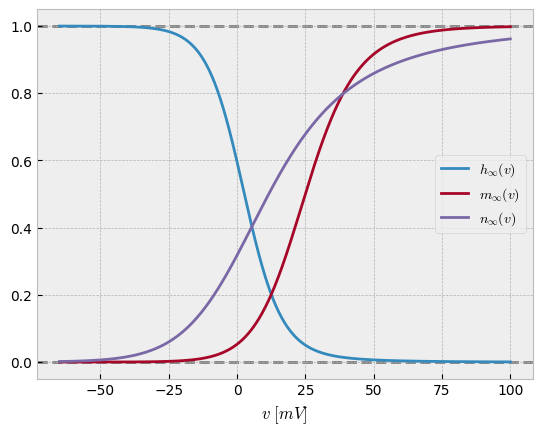
\includegraphics[width=0.35\textwidth]{figs/ej2_fracciones.png}
    \caption{Valor de equilibrio de fracción de compuertas de activación e inactivación abiertas en función del potencial de membrana.}
    \label{fig:ej2_fracciones}
\end{figure}

A simple vista, notamos que las compuertas de activación se abren al aumentar el potencial de membrana, mientras que las de inactivación se cierran.

Podemos observar que para un potencial de membrana de entre aproximadamente -20 mV y 50 mV, va a haber flujo de iones de sodio a través de los canales correspondientes ya que para estos valores de voltaje se cumple que hay tanto compuertas de activación como de inactivación abiertas. Para valores de potencial de membrana menores a -20 mV las compuertas de activación del sodio están cerradas, mientras que para valores mayores a 50 mV las compuertas de inactivación del sodio están cerradas; y en ninguno de los dos casos va a haber flujo de iones de sodio.

Por otro lado, la apertura de los canales de potasio se comienza a dar cuando el voltaje es de al menos -50 mV. Además, a partir de los 150 mV aproximadamente es que se llega a todas las compuertas de activación del potasio abiertas. 

\begin{figure}[ht]
    \centering
    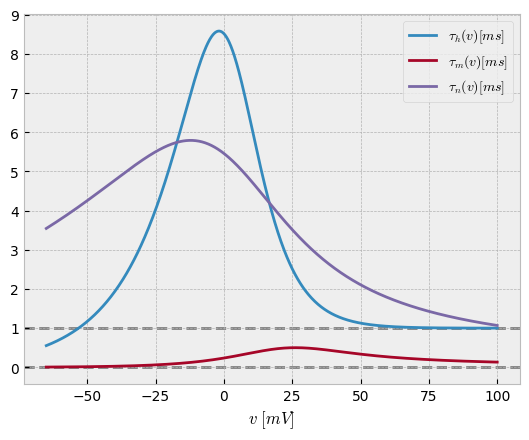
\includegraphics[width=0.35\textwidth]{figs/ej2_tiempos-caracteristicos.png}
    \caption{Tiempos característicos de las compuertas de activación e inactivación abiertas.} 
    \label{fig:ej2_tiempos-caracteristicos}
\end{figure}

En este gráfico, podemos observar que para todos los valores de voltaje medidos, el tiempo característico de $m$ (\(\tau_m\)) es cercano a 0, indicando que las compuertas de activación del sodio responden rápido a cambios de potencial en la membrana, llegando casi instantáneamente a su valor de equilibrio. 

Analizando (\(\tau_n\)), vemos que para un voltaje positivo, a medida que es mayor $n$ cada vez tarda menos en llegar a su valor de equilibrio, acercándose asintóticamente a 0 segundos. Es decir, a mayor voltaje positivo, las compuertas responden cada vez más rápido a diferencias en el potencial de membrana.

Finalmente examinando (\(\tau_h\)), vemos que $h$ va a tardar la mayor cantidad de tiempo en alcanzar su valor de equilibrio cuando el potencial de la membrana es de aproximadamente 0 mV. A medida que aumenta el valor absoluto del potencial de membrana, va a disminuir el tiempo característico, acercándose asintóticamente a 0 ms para voltaje negativo y a 1 ms para voltaje positivo. 

A continuación comenzamos con las simulaciones del potencial de membrana y las fracciones de compuertas abiertas en el tiempo dados distintos estímulos de corriente externa.

Siguiendo lo observado en estos primeros dos gráficos, esperamos ver en general que partiendo del potencial de reposo, al introducir una corriente externa el potencial de membrana aumenta y las fracciones de compuertas abiertas buscan ir a su valor de equilibrio correspondiente según \ref{fig:ej2_fracciones}, y a la velocidad acorde a lo presentado en \ref{fig:ej2_tiempos-caracteristicos}.

\subsection{Valores de equilibrio}
Condiciones iniciales: $h_0 = m_0 = n_0 = 0$

Corriente externa: $i(t) = 0\mu A/cm^2 \ \forall t$

\begin{figure}[ht]
    \centering
    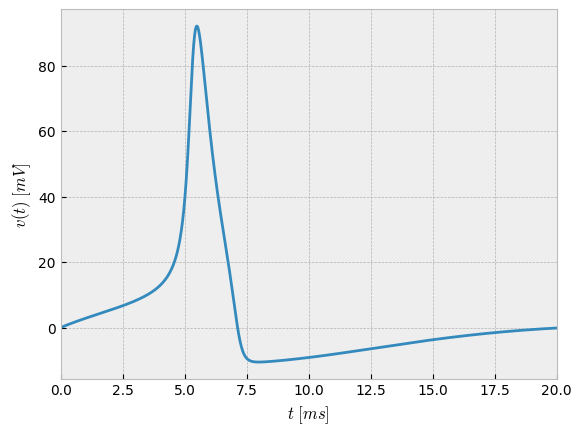
\includegraphics[width=0.35\textwidth]{figs/ej3_potencial.png}
    \caption{Potencial de membrana en función del tiempo.} 
    \label{fig:ej3_potencial}
\end{figure}
\begin{figure}[ht]
    \centering
    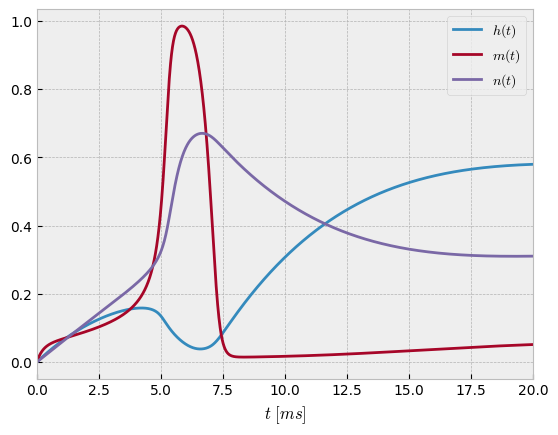
\includegraphics[width=0.35\textwidth]{figs/ej3_canales.png}
    \caption{Canales de activación e inactivación en función del tiempo.} 
    \label{fig:ej5_canales}
\end{figure}

Es importante resaltar que aquí ninguna señal externa está siendo transmitida y que inicialmente $n$, $m$ y $h$ están en 0. Lo que ocurre entonces es que las compuertas comienzan a abrirse, intentando alcanzar sus respectivos valores de equilibrio dado el voltaje. Esta apertura genera un aumento progresivo del potencial de membrana hasta aproximadamente los 15mV, punto en el cual se genera una rápida apertura de los canales de activación de sodio ($m$) al mismo tiempo que los canales de inactivación de sodio ($h$) alcanzan su mínimo, causando que el potencial de membrana produzca un pico hasta llegar aproximadamente a los 95mV. Mientras $m$ va creciendo, la fracción de canales de potasio abiertos ($n$) también lo hace, aunque un poco más lentamente y, junto con el paulatino incremento de $h$ posterior al pico de $m$ - lo cual reduce el flujo de iones de sodio-, contribuyen a que disminuya el voltaje. De esta forma, se produce una caída en el potencial de membrana que a su vez va cerrando las compuertas de activación de los canales de sodio y también las compuertas de activación del potasio. Vemos también que el voltaje cae hasta un valor más bajo que el de reposo y luego se reacomoda, a medida que $h$, $m$, $n$ alcanzan sus valores de equilibrio, correspondientes a los vistos en el primer gráfico, los cuales son:
\begin{eqnarray}
h^* &\approx 0.3184 \nonumber\\
m^* &\approx 0.0532 \nonumber\\
n^* &\approx 0.5945 \nonumber
\end{eqnarray}

\subsection{Estímulo débil y estímulo fuerte}
Condiciones iniciales: valores de equilibrio hallados en el experimento 2.

Corriente externa:
$$
i(t) = \left\{
\begin{array}{ll}
10 \mu A/cm^2, & t\in [2ms,2.5ms] \\
30 \mu A/cm^2, & t\in [10ms,10.5ms] \\
0 \mu A/cm^2, & c.c. \\
\end{array}
\right.
$$

\begin{figure}[ht]
    \centering
    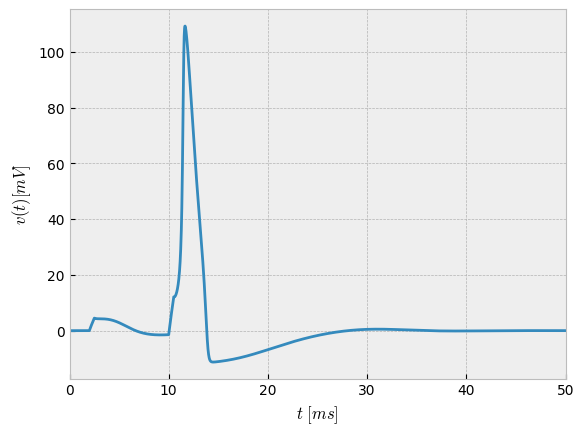
\includegraphics[width=0.35\textwidth]{figs/ej4_potencial.png}
    \caption{Potencial de membrana en función del tiempo.} 
    \label{fig:ej4_potencial}
\end{figure}
\begin{figure}[ht]
    \centering
    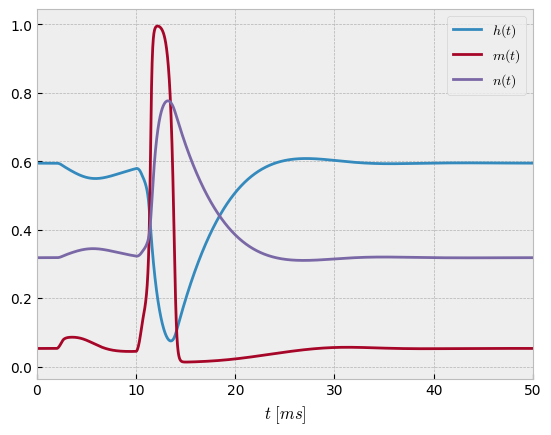
\includegraphics[width=0.35\textwidth]{figs/ej4_canales.png}
    \caption{Canales de activación e inactivación en función del tiempo.} 
    \label{fig:ej4_canales}
\end{figure}

Notemos primero que, a diferencia del experimento anterior, al comenzar en los valores de equilibrio de $h$, $n$, $m$ y $v$ y con una corriente nula hasta el milisegundo 2, todo se mantiene invariante hasta dicho momento.

Ahora bien, se puede observar que el primer pico de corriente externa de 10 $\mu A/cm^2$ no es suficiente como para provocar una alteración significativa en el potencial de membrana, el cual sube levemente y vuelve a su reposo. Sin embargo, más tarde se presenta otro estímulo pero esta vez mayor, de 30 $\mu A/cm^2$, y suficiente para generar un potencial de acción, prácticamente igual al observado en el ensayo anterior.

\subsection{Ráfaga}
Condiciones iniciales: valores de equilibrio hallados en el experimento 2.

Corriente externa:
$$
i(t) = \left\{
\begin{array}{ll}
10 \mu A/cm^2, & t\in [5ms,\infty ms) \\
0 \mu A/cm^2, & c.c. \\
\end{array}
\right.
$$

\begin{figure}[ht]
    \centering
    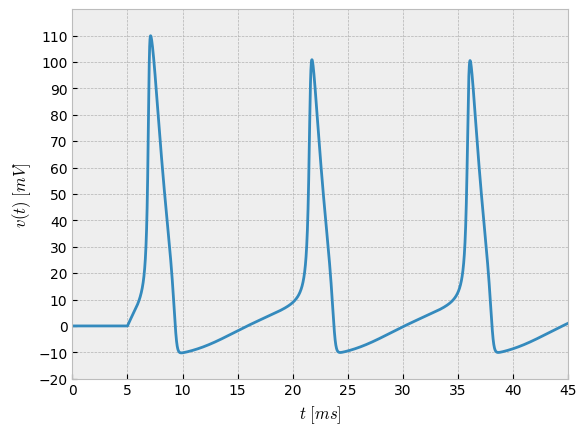
\includegraphics[width=0.35\textwidth]{figs/ej5_potencial.png}
    \caption{Potencial de membrana en función del tiempo.} 
    \label{fig:ej5_potencial}
\end{figure}
\begin{figure}[ht]
    \centering
    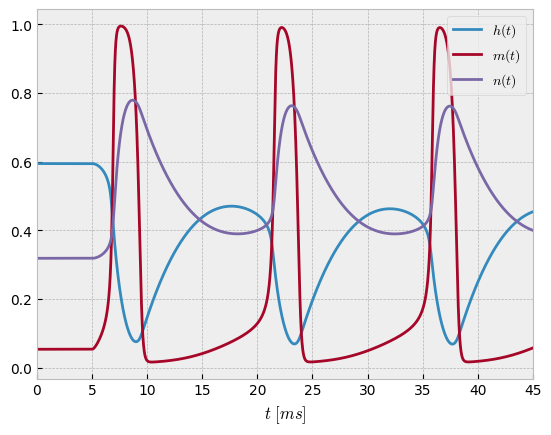
\includegraphics[width=0.35\textwidth]{figs/ej5_canales.png}
    \caption{Canales de activación e inactivación en función del tiempo.} 
    \label{fig:ej5_canales}
\end{figure}

El comportamiento observado al comenzar el estímulo sigue lo presentado en el experimento anterior al darse el estímulo fuerte. Al utilizarse en este caso un estímulo constante, la dinámica se va a repetir periódicamente, en forma de ráfaga. Podemos notar que luego del primer pico, $h$ no alcanza a volver a su valor inicial de equilibrio, se mantiene siempre más bajo. Esto provoca que el ingreso de iones de sodio nunca será tan alto como cuando comenzó el estímulo externo a los 5 ms, con lo cual los picos de voltaje siguientes al primero serán todos un poco más bajos que este. 


\subsection{Período refractario}
Condiciones iniciales: valores de equilibrio hallados en el experimento 2.

Corriente externa:
$$
i(t) = \left\{
\begin{array}{ll}
10 \mu A/cm^2, & t\in [10ms\, k,10 ms\, k + 2ms], \\
& k \in \{1,2,3,4,5,...\}\\
0 \mu A/cm^2, & c.c. \\
\end{array}
\right.
$$

\begin{figure}[ht]
    \centering
    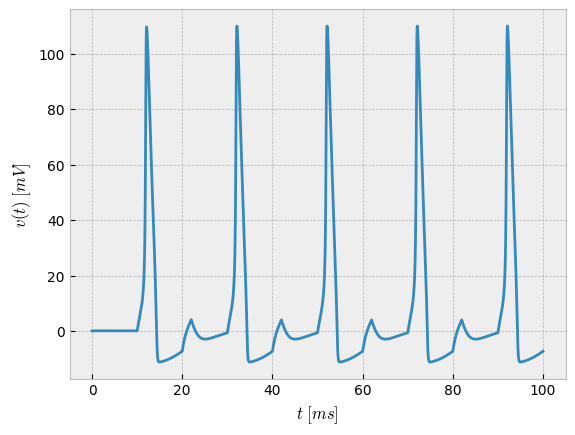
\includegraphics[width=0.35\textwidth]{figs/ej6_potencial.png}
    \caption{Potencial de membrana en función del tiempo.} 
    \label{fig:ej6_potencial}
\end{figure}
\begin{figure}[ht]
    \centering
    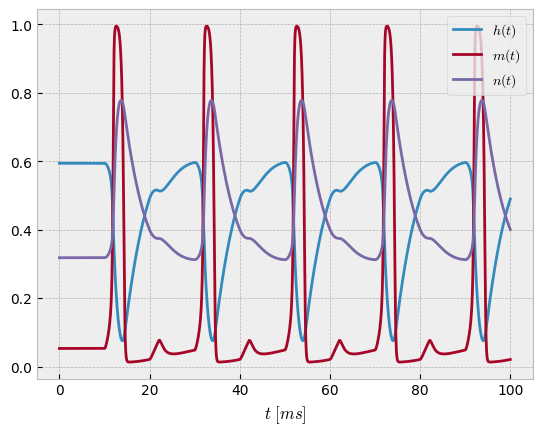
\includegraphics[width=0.35\textwidth]{figs/ej6_canales.png}
    \caption{Canales de activación e inactivación en función del tiempo.} 
    \label{fig:ej6_canales}
\end{figure}

En este experimento se observan dos picos de corriente por cada período de activación; el primero se da cuando el potencial de membrana se encuentra en reposo, y observamos cómo se activa la neurona, y el segundo se da cuando el potencial está por debajo de su valor de reposo, y no es suficiente para superar el umbral de apertura de los canales de sodio, responsables del pico de potencial. A este lapso en el cual la membrana está retornando a su potencial de reposo luego de una caída y en el cual se necesitaría un estímulo mayor para efectuar el disparo se lo conoce como período \textit{refractario}.

\subsection{Excitaciones espontáneas en respuesta al ruido}
Condiciones iniciales: valores de equilibrio hallados en el experimento 2.

Corriente externa: $i(t)\sim i_0 N(0,1)$ (i.e. $i_0$ multiplicado por un valor aleatorio obtenido de una distribución normal de media 0 y varianza 1) para cada valor de $t$ en el que sea evaluada. Tomamos $i_0=50\mu A$.

\begin{figure}[ht]
    \centering
    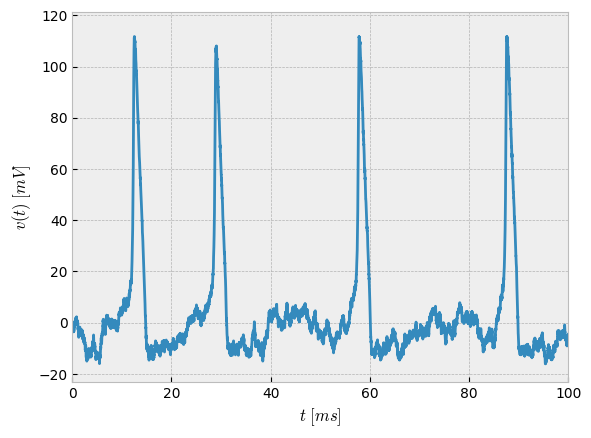
\includegraphics[width=0.35\textwidth]{figs/ej7_potencial.png}
    \caption{Potencial de membrana en función del tiempo.} 
    \label{fig:ej7_potencial}
\end{figure}
\begin{figure}[ht]
    \centering
    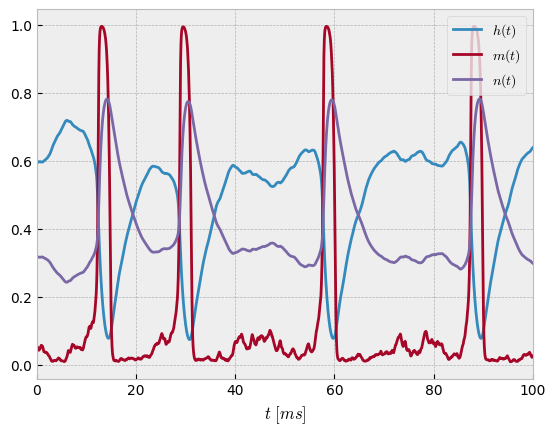
\includegraphics[width=0.35\textwidth]{figs/ej7_canales.png}
    \caption{Canales de activación e inactivación en función del tiempo.} 
    \label{fig:ej7_canales}
\end{figure}

La aleatoriedad introducida en la corriente genera que la trayectoria de estas funciones del tiempo no sea periódica, y muy dependiente de la amplitud $i_0$, aunque se puede asumir que en promedio hay picos de activación cada 21.34 ms, con un máximo período de 34.55 ms. Nuevamente observamos la presencia del periodo refractario, en el que hay estímulo externo pero no es suficiente para que dispare la neurona. 

\section{Discusión}
En los distintos experimentos pudimos observar la relación entre los estímulos de corriente externa, el potencial de membrana y las fracciones de compuertas de activación e inactivación en cada unidad de tiempo, permitiéndonos entender el período de activación del potencial como el producto de corrientes a través de la membrana. En todos los casos de estudio pudimos observar cuatro fases bien definidas que explican la cinética del potencial de membrana tras el equilibrio:

\textit{Despolarización}. Período en el que el potencial supera un umbral tal que la fracción y la velocidad de apertura de compuertas de activación de sodio es mayor que la de la apertura de las compuertas de potasio y la del cierre de las de inactivación de sodio, permitiendo el ingreso predominante de iones de sodio a la membrana, provocando el pico en el potencial de acción.

\textit{Repolarización}. Período en el cual la fracción de compuertas de inactivación del sodio cerradas y las de activación del potasio abiertas predominan, de manera que se detiene el flujo de iones de sodio y la célula vuelve rápidamente a su estado de equilibrio gracias a la corriente de iones de potasio hacia el exterior.

\textit{Hiperpolarización}. Período corto de tiempo en el que el potencial pasa por debajo de su valor de equilibrio debido a que la fracción de compuertas de activación de potasio es tal que permite continuar el flujo de iones al exterior de la célula, mientras que las compuertas de sodio permanecen cerradas.

\textit{Estabilización}. Período de normalización del potencial de membrana, donde se puede ver cómo el potencial vuelve gradualmente al equilibrio, junto con los valores de equilibrio de las fracciones de compuertas.

Cada vez que la corriente externa permita que el potencial crezca gradualmente hasta superar un umbral de activación de los canales de sodio, comienza nuevamente la despolarización y se repiten las etapas mencionadas anteriormente.

En general, en todos los experimentos vemos que  $m$ es prácticamente proporcional al potencial adquirido en todo momento, y cómo $h$ es proporcionalmente inversa a $n$.

\section{Conclusiones}
Podemos concluir que la simulación del modelo de Hodgkin-Huxley con nuestros experimentos nos permite visualizar claramente los distintos fenómenos electroquímicos que describe la neurona para transmitir señales eléctricas a lo largo del axón. En todos los casos de estudio se pueden diferenciar bien cuatro etapas que caracterizan el período de activación del potencial; la despolarización de la membrana a partir de la corriente predominante de iones de sodio a través de la membrana, la repolarización tras la corriente de potasio que expulsa la célula, un período de hiperpolarización producido por la velocidad baja de cierre de las compuertas de potasio frente a las de sodio y un período de estabilización consecuencia de la corriente residual en la membrana. Este análisis explica gráficamente cómo la cinética de las fracciones de compuertas sensibles al voltaje y el potencial se retroalimentan para llevar a cabo la propagación del potencial de acción tras estímulos de corriente externa.

% If in two-column mode, this environment will change to single-column
% format so that long equations can be displayed. Use
% sparingly.
%\begin{widetext}
% put long equation here
%\end{widetext}

% figures should be put into the text as floats.
% Use the graphics or graphicx packages (distributed with LaTeX2e)
% and the \includegraphics macro defined in those packages.
% See the LaTeX Graphics Companion by Michel Goosens, Sebastian Rahtz,
% and Frank Mittelbach for instance.
%
% Here is an example of the general form of a figure:
% Fill in the caption in the braces of the \caption{} command. Put the label
% that you will use with \ref{} command in the braces of the \label{} command.
% Use the figure* environment if the figure should span across the
% entire page. There is no need to do explicit centering.

% \begin{figure}
% \includegraphics{}%
% \caption{\label{}}
% \end{figure}

% Surround figure environment with turnpage environment for landscape
% figure
% \begin{turnpage}
% \begin{figure}
% \includegraphics{}%
% \caption{\label{}}
% \end{figure}
% \end{turnpage}

% tables should appear as floats within the text
%
% Here is an example of the general form of a table:
% Fill in the caption in the braces of the \caption{} command. Put the label
% that you will use with \ref{} command in the braces of the \label{} command.
% Insert the column specifiers (l, r, c, d, etc.) in the empty braces of the
% \begin{tabular}{} command.
% The ruledtabular enviroment adds doubled rules to table and sets a
% reasonable default table settings.
% Use the table* environment to get a full-width table in two-column
% Add \usepackage{longtable} and the longtable (or longtable*}
% environment for nicely formatted long tables. Or use the the [H]
% placement option to break a long table (with less control than 
% in longtable).
% \begin{table}%[H] add [H] placement to break table across pages
% \caption{\label{}}
% \begin{ruledtabular}
% \begin{tabular}{}
% Lines of table here ending with \\
% \end{tabular}
% \end{ruledtabular}
% \end{table}

% Surround table environment with turnpage environment for landscape
% table
% \begin{turnpage}
% \begin{table}
% \caption{\label{}}
% \begin{ruledtabular}
% \begin{tabular}{}
% \end{tabular}
% \end{ruledtabular}
% \end{table}
% \end{turnpage}

%\section{Aknowledgments}
\section{Agradecimientos}
Agradecemos a FAMAF y a la cátedra por motivarnos, y darnos el espacio y las herramientas para llevar a cabo este proyecto. 
% Create the reference section using BibTeX:
\bibliographystyle{apsrev4-2}
\bibliography{refs}

% Specify following sections are appendices. Use \appendix* if there
% only one appendix.
\end{document}
%
% ****** End of file apstemplate.tex ******


